\appendix
\section{Voting Interface Breakdown}\label{apdx:relatedVoting}
\paragraph{Designs that shifted voter decisions: } For example, states without straight-party ticket voting~(where voters can select all candidates from one party through a single choice) exhibited higher rates of split-ticket voting~\cite{engstrom2020politics}. Another example from the Australian ballot showing incumbency advantages is where candidates are listed by the office they are running for, with no party labels or boxes.
\paragraph{Designs that influenced errors: } Butterfly ballots increased voter errors because voters could not correctly identify the punch hole on the ballot. Splitting contestants across columns increases the chance for voters to overvote~\cite{quesenberyOpinionGoodDesign2020}. On the other hand, \textcite{everettElectronicVotingMachines2008} showed the use of incorporating physical voting behaviors, like lever voting, into graphical user interfaces.
\paragraph{Designs that incorporated technologies: } Other projects like the Caltech-MIT Voting Technology Project have sparked research to address accessibility challenges, resulting in innovations like EZ Ballot~\cite{leeUniversalDesignBallot2016}, Anywhere Ballot~\cite{summers2014making}, and Prime III~\cite{dawkinsPrimeIIIInnovative2009}. In addition, \textcite{gilbertAnomalyDetectionElectronic2013} investigated optimal touchpoints on voting interfaces, and \textcite{conradElectronicVotingEliminates2009} examined zoomable voting interfaces.


\section{Interface design process}\label{apdx:design}
In this section, we outline the design process leading to our final interface. As mentioned in the paper, our design iteration is based on existing QV applications in the wild.

\begin{figure}[H]
    \centering
    \begin{subfigure}[b]{0.54\textwidth}
        \centering
        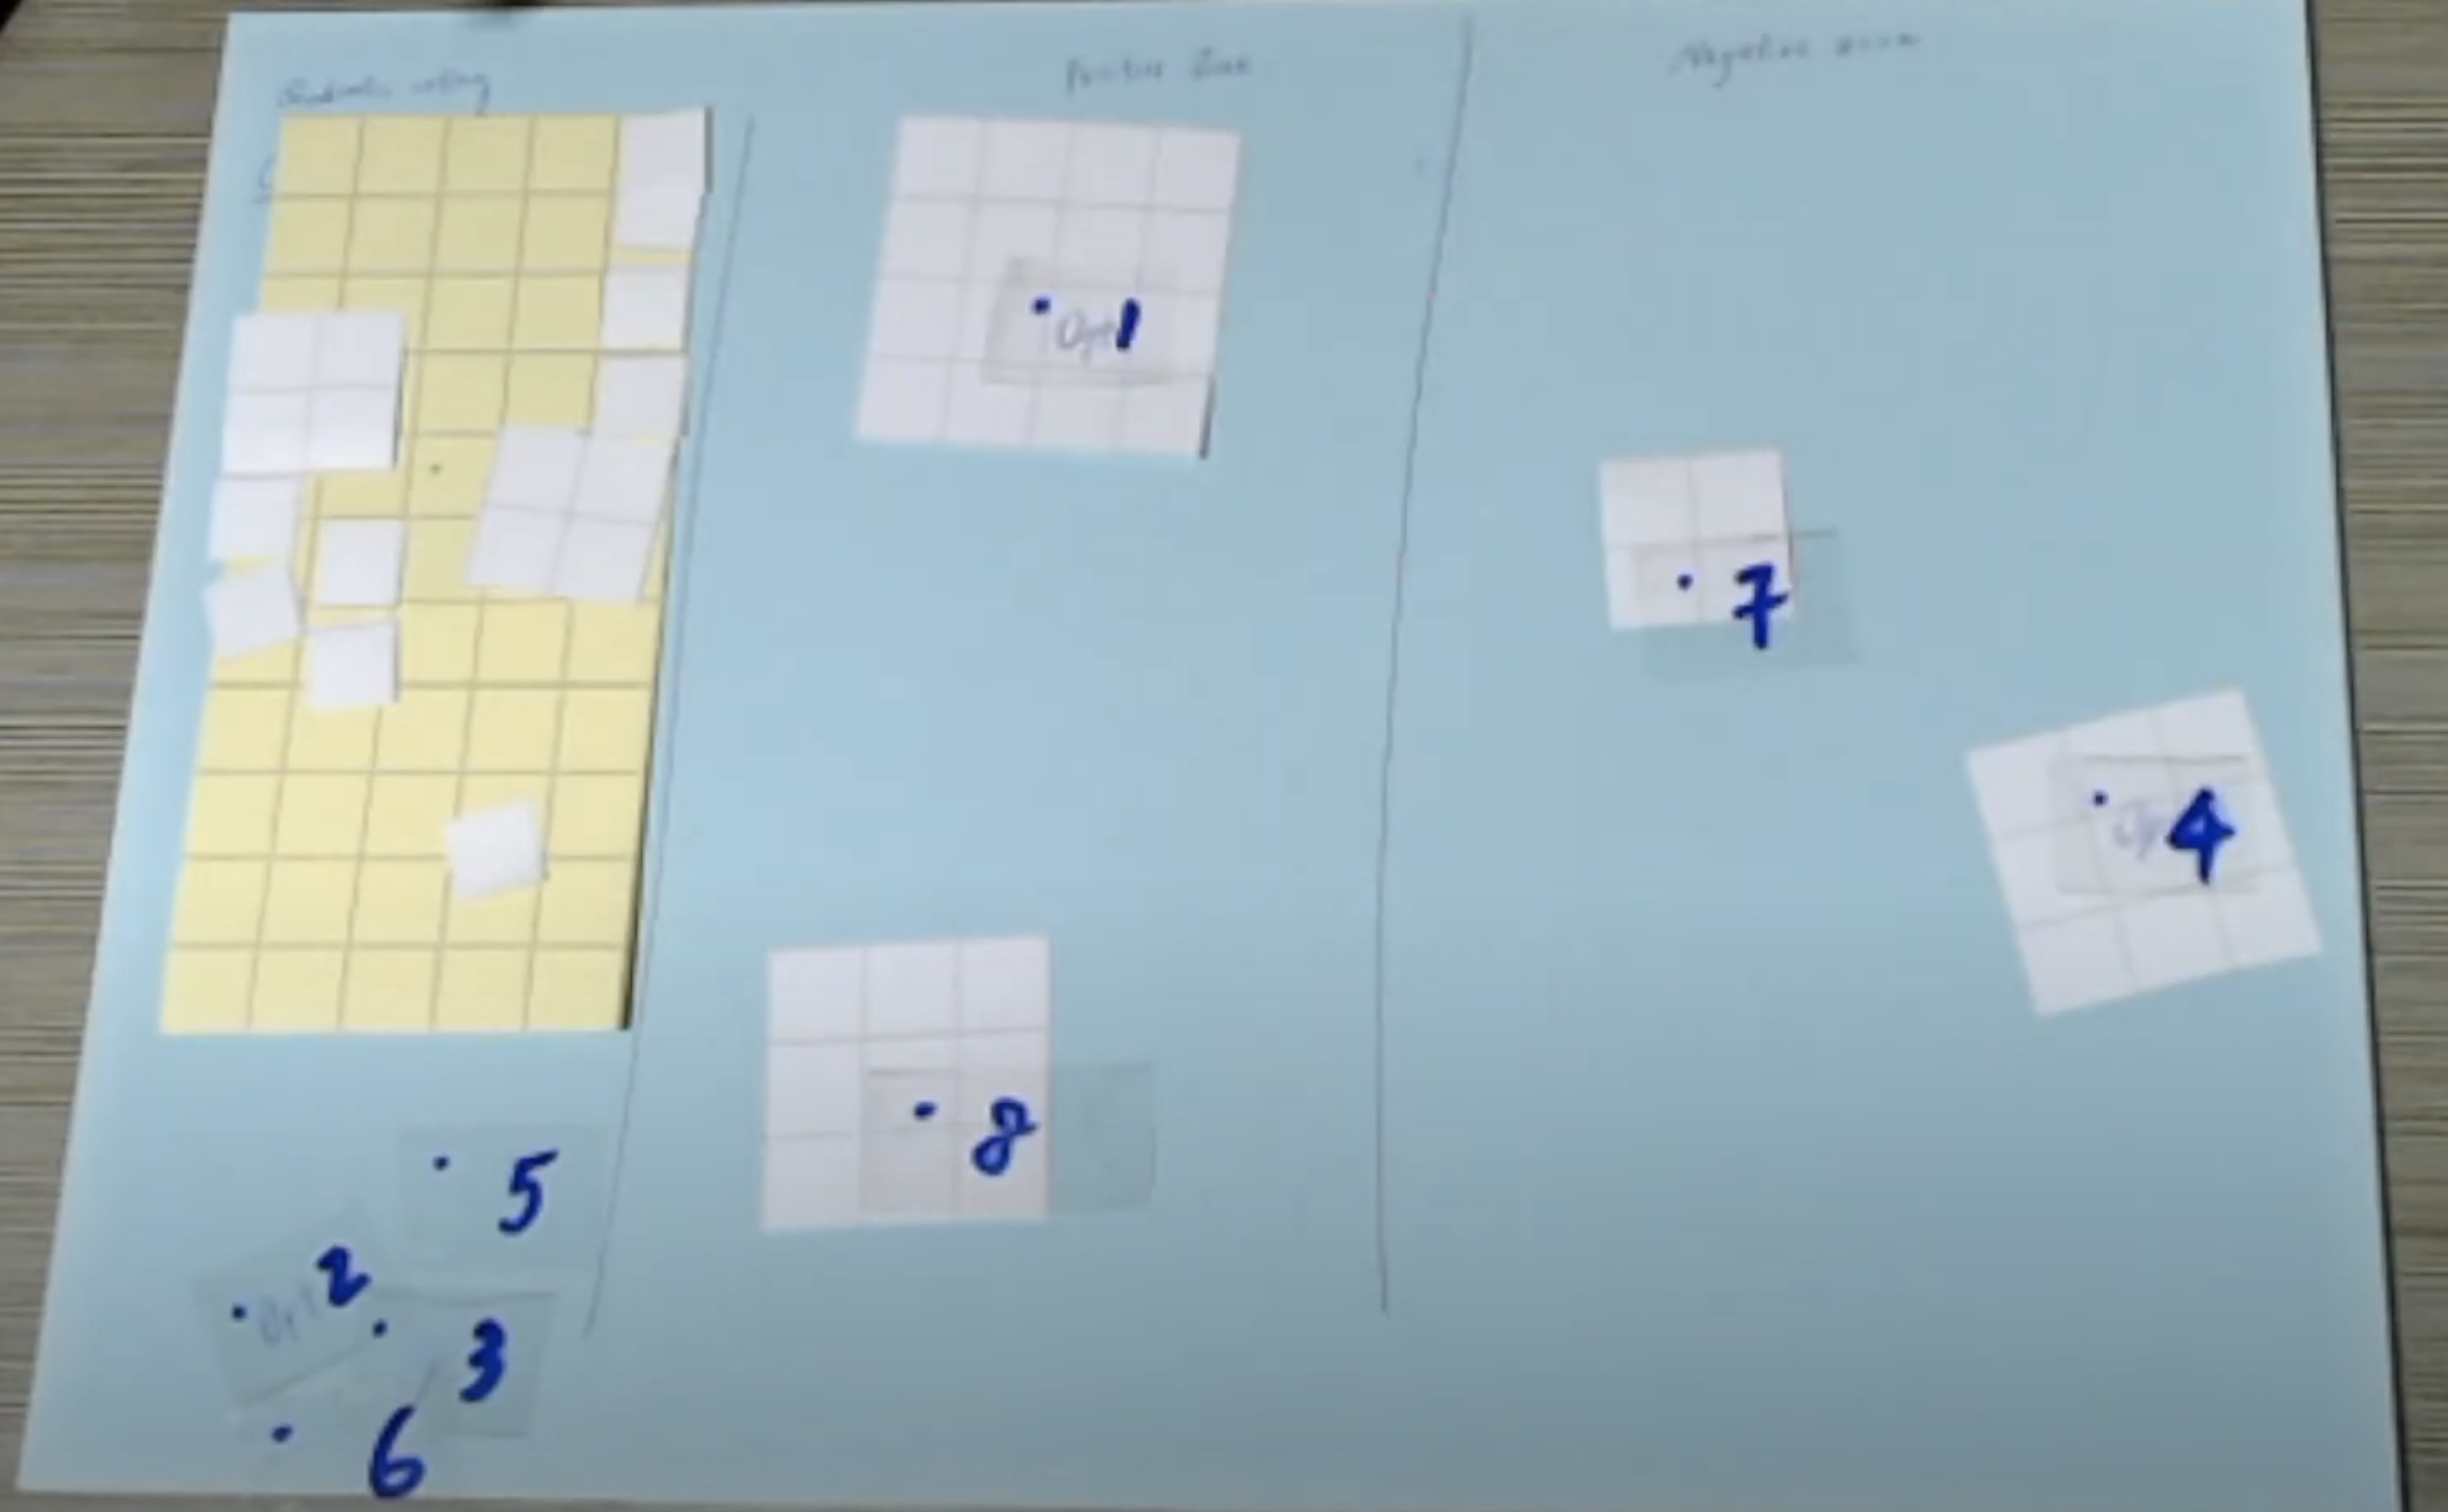
\includegraphics[width=\textwidth]{content/image/prototypes/1.2_paper_qv_single.png}
        \caption{In this paper prototype, issues are denoted by different numbers that appear on mouseover. Pretest respondents can move options anywhere in the two sections of the interface, one denoting positive and one negative. The blocks represent the cost for each option, with no indication of the number of current votes. The credits are shown in the yellow box on the left.}
        \label{fig:horizontal_paper}
    \end{subfigure}
    \hfill
    \begin{subfigure}[b]{0.42\textwidth}
        \centering
        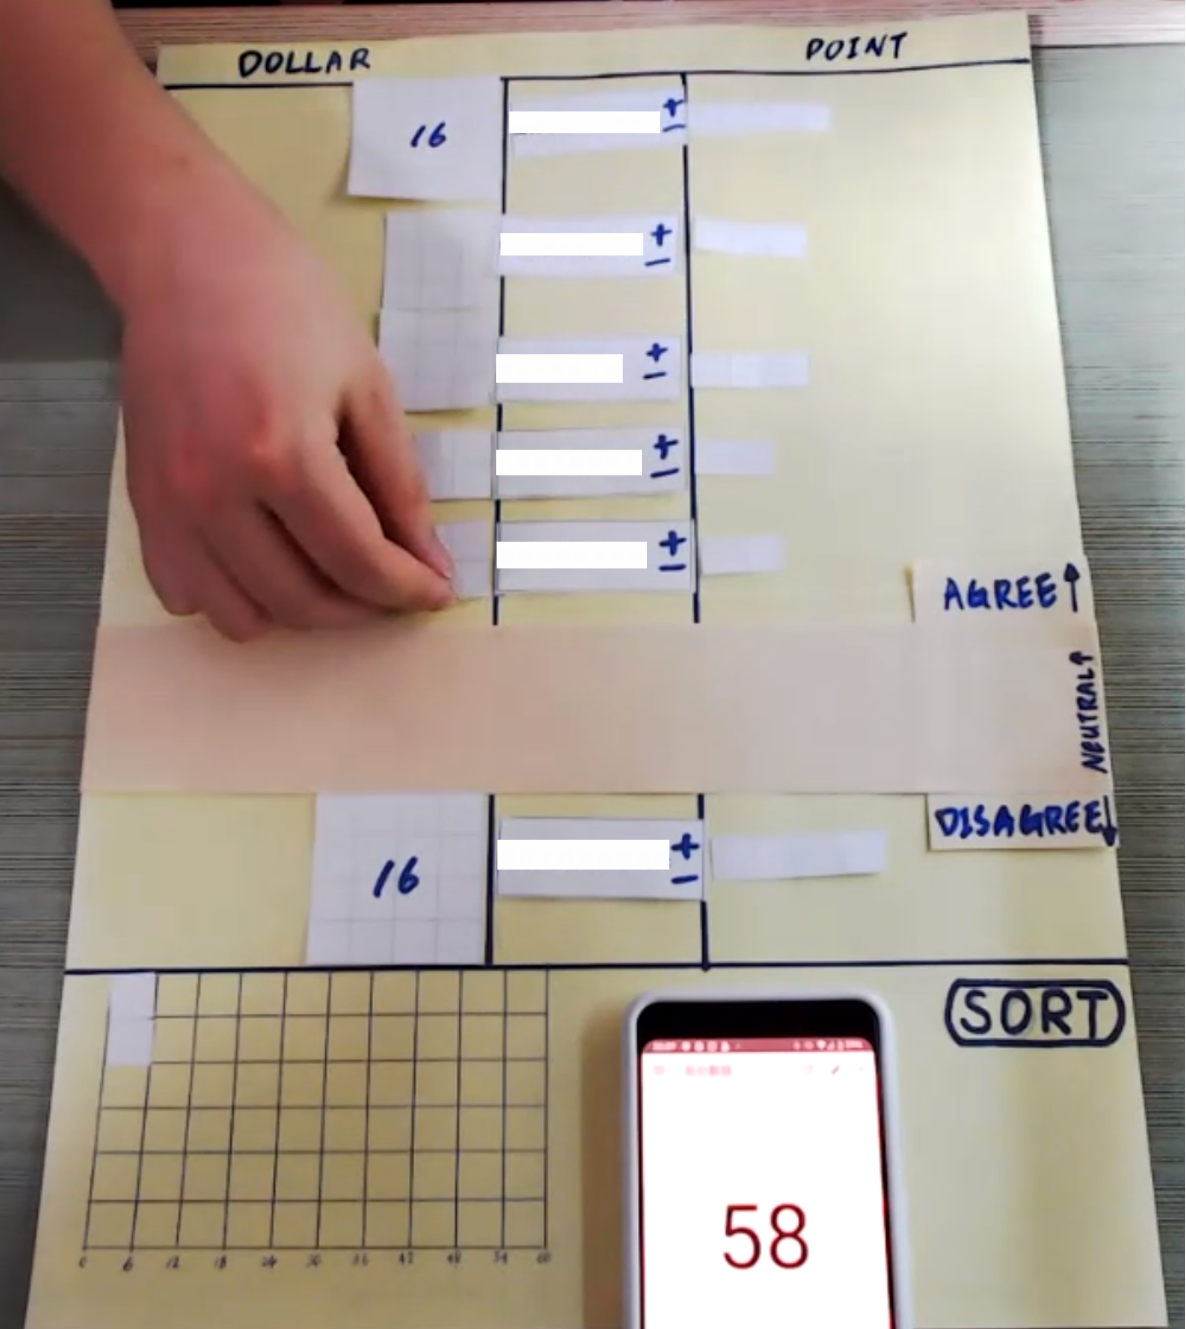
\includegraphics[width=\textwidth]{content/image/prototypes/1_paper_qv_single.png}
        \caption{This paper prototype separates the positive and negative areas with a 'band' at the center. Undecided options are placed inside this band. The cost and the votes on both sides of the interface are denoted by small blocks. The budget is shown in the yellow box below the interface with a numerical counter.}
        \label{fig:vertical_paper}
    \end{subfigure}
    \caption{Initial paper prototypes designed for QS interface}
    \label{fig:qv_paper}
\end{figure}

\subsubsection{Prototype 1: Ranking-Vote}
Considering that relative preference is often through ranking items, we tested whether ranking options before voting would help establish an individual's relative preference in our prototype 1. This prototype allowed respondents to reposition options before voting. Pretests revealed that respondents rarely moved the options and questioned the necessity of full ranking, as it did not influence their QS submission. Additionally, many were unaware that options were draggable until shown. This insight indicates that full ranking is unnecessary for establishing relative preferences. Therefore, we decided to ask respondents to select a subset of options instead of requiring a full rank among all options.

\begin{figure}[h]
    \centering
    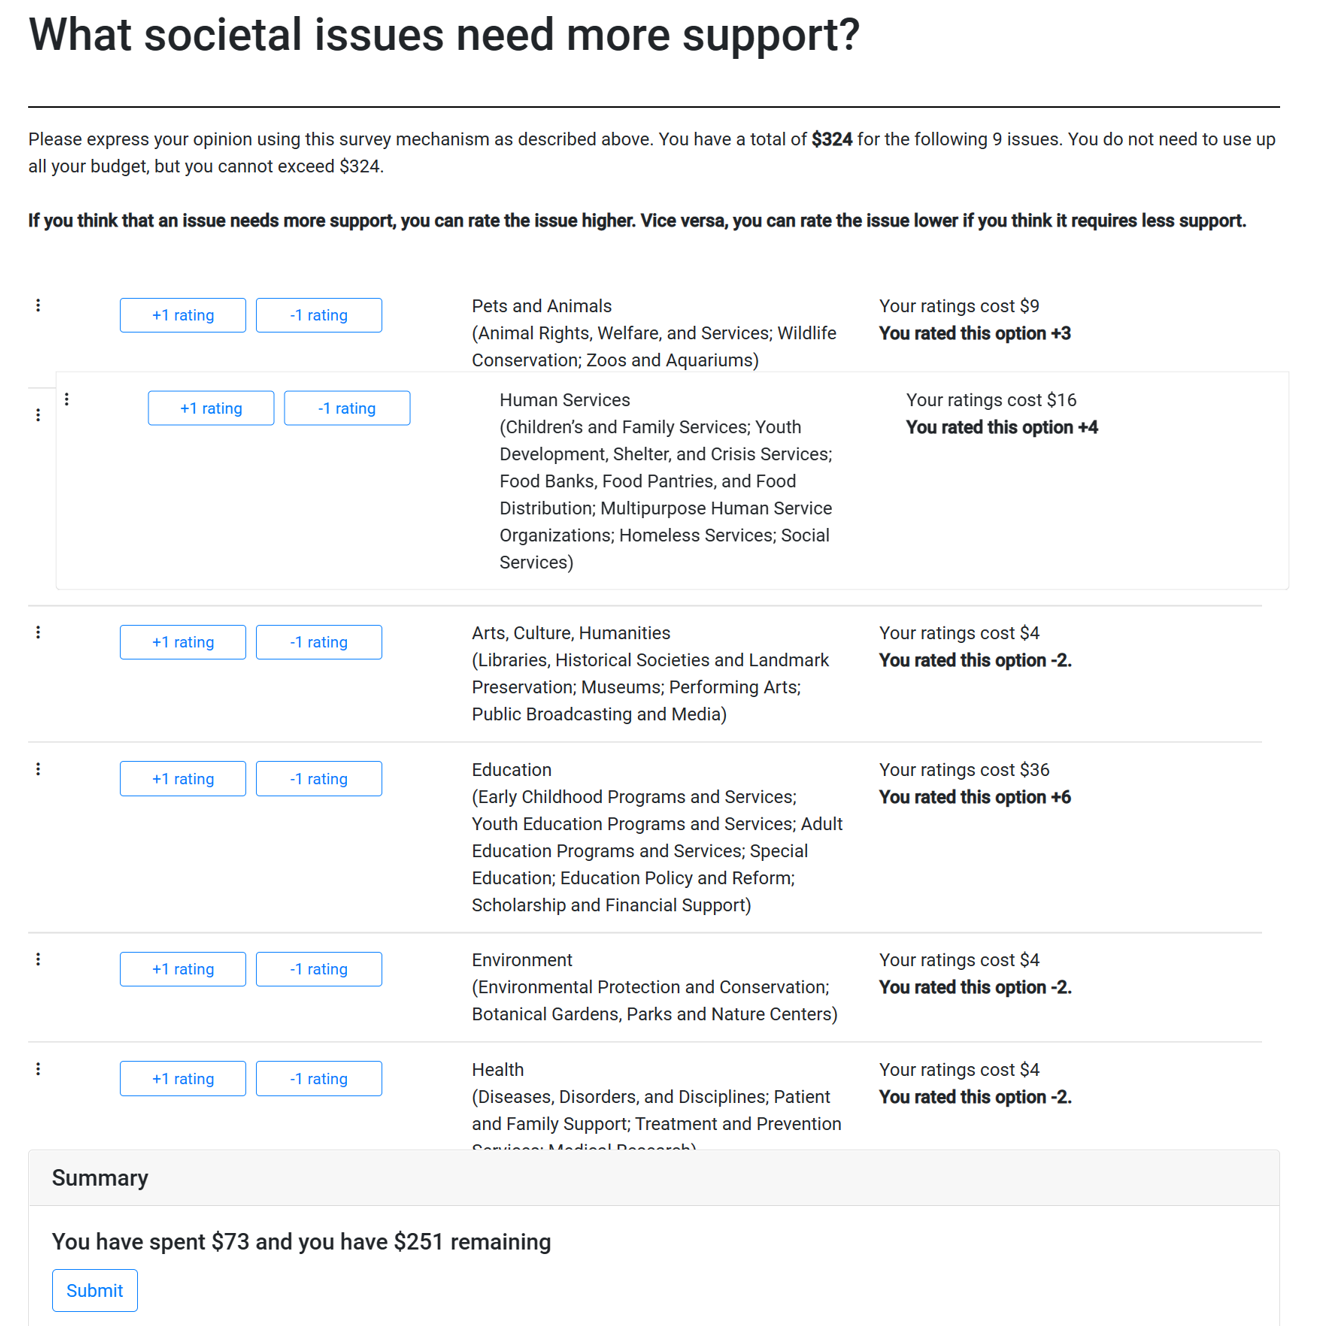
\includegraphics[width=0.43\textwidth]{content/image/prototypes/2_ranking.png}
    \caption{A Ranking-Vote Prototype: The goal of this prototype is to test whether ranking options prior to voting help establish an individual's relative preferences and reduce effort when voting. Each option is draggable to position in a specific location amongst the full list of options. Votes can be updated using the buttons to the right of the interface with vote count and costs to the right of the interface. A summary box is placed sticky to the bottom of the screen.}
    \label{fig:qv_rank}
\end{figure}

\begin{figure}[h]
    \centering
    \begin{subfigure}[b]{0.47\textwidth}
        \centering
        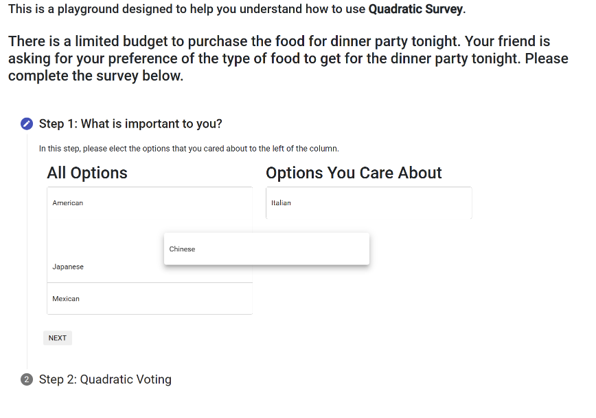
\includegraphics[width=0.9\textwidth]{content/image/prototypes/3.1_selecting.png}
        \caption{Options are dragged and dropped to the 'Option You Care About' box.}
        \label{fig:qv_select_selection}
    \end{subfigure}
    \hfill
    \begin{subfigure}[b]{0.47\textwidth}
        \centering
        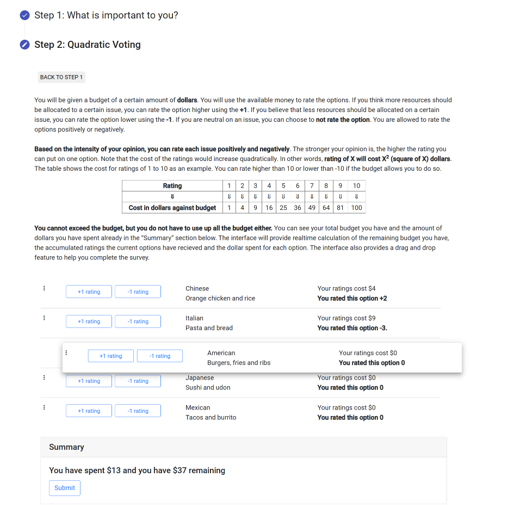
\includegraphics[width=0.9\textwidth]{content/image/prototypes/3.2_selecting_2.png}
        \caption{The previous step collapses showing all voting options.}
        \label{fig:qv_select_vote}
    \end{subfigure}
    \caption{A Select-then-Vote Prototype: The goal of this prototype is to nudge participants to focus on a subset of options to vote, rather than ranking all of them. This prototype introduces a two-step voting process. As shown in Fig.~\ref{fig:qv_select_selection}, the first step involves selecting options for further consideration. Important options are placed at the top of the list for voting shown in Fig.~\ref{fig:qv_select_vote}, but options can be placed anywhere on the list if desired. The rest of the controls remain the same as the previous prototype.}
    \label{fig:qv_select}
\end{figure}

\subsubsection{Prototype 2: Select-then-Vote}
Based on feedback from Prototype 1, instead of \textit{allowing} individuals to rank options, Prototype 2 implemented a two-phase process that \textit{intentionally} asks respondents to select options to express opinions before voting. As shown in Figure~\ref{fig:qv_select}, survey respondents selected their preferred options (Figure~\ref{fig:qv_select_selection}), and the interface positioned these options at the top of the list for voting (Figure~\ref{fig:qv_select_vote}). We identified several issues during the prototype 2 pretest: many respondents marked most options as 'options they care about,' which undermined the design's purpose. Additionally, the lack of clear distinction between selected and unselected options confused respondents about the necessity of Step 1. Thus, we need a clearer distinction and connection between the two phases to effectively construct relative preferences.

\begin{figure}[h]
    \centering
    \begin{subfigure}[b]{0.48\textwidth}
        \centering
        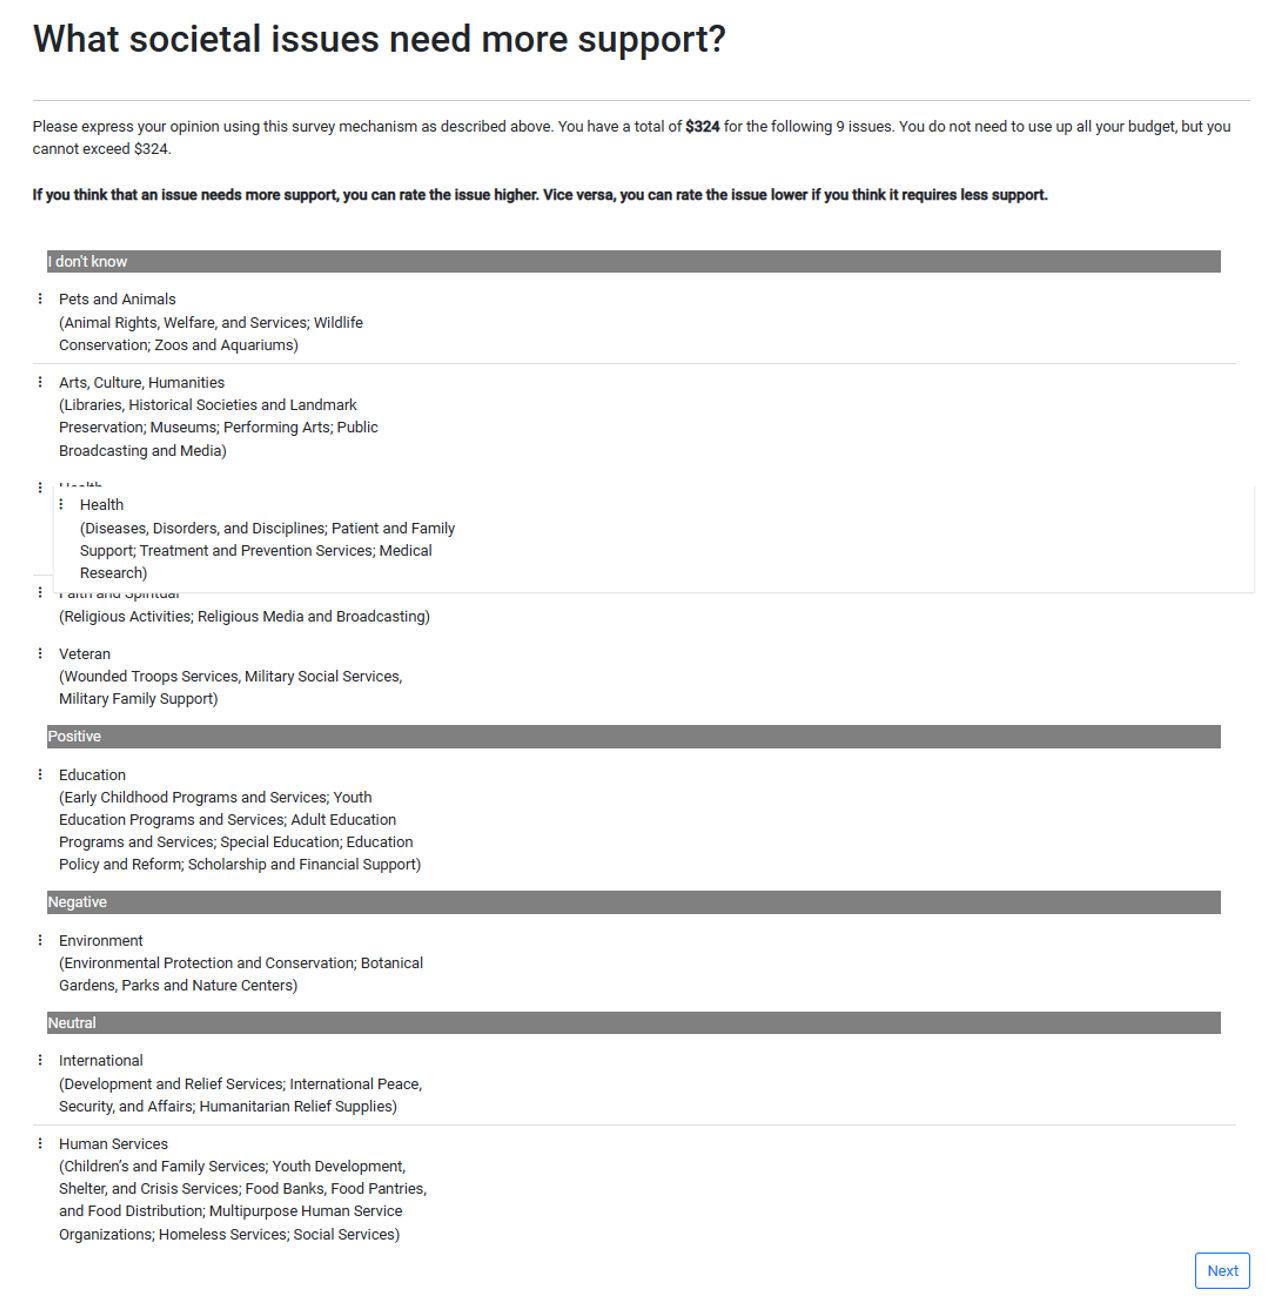
\includegraphics[width=\textwidth]{content/image/prototypes/4.1_grouping.png}
        \caption{The Organization Interface: Options are shown initially in the first bin labeled as `I don't know.' Survey respondents can then drag and drop these options into the latter bins: Positive, Neutral, or Negative. Only the details of each option are shown on this interface.}
        \label{fig:qv_org_p1}
    \end{subfigure}
    \hfill
    \begin{subfigure}[b]{0.48\textwidth}
        \centering
        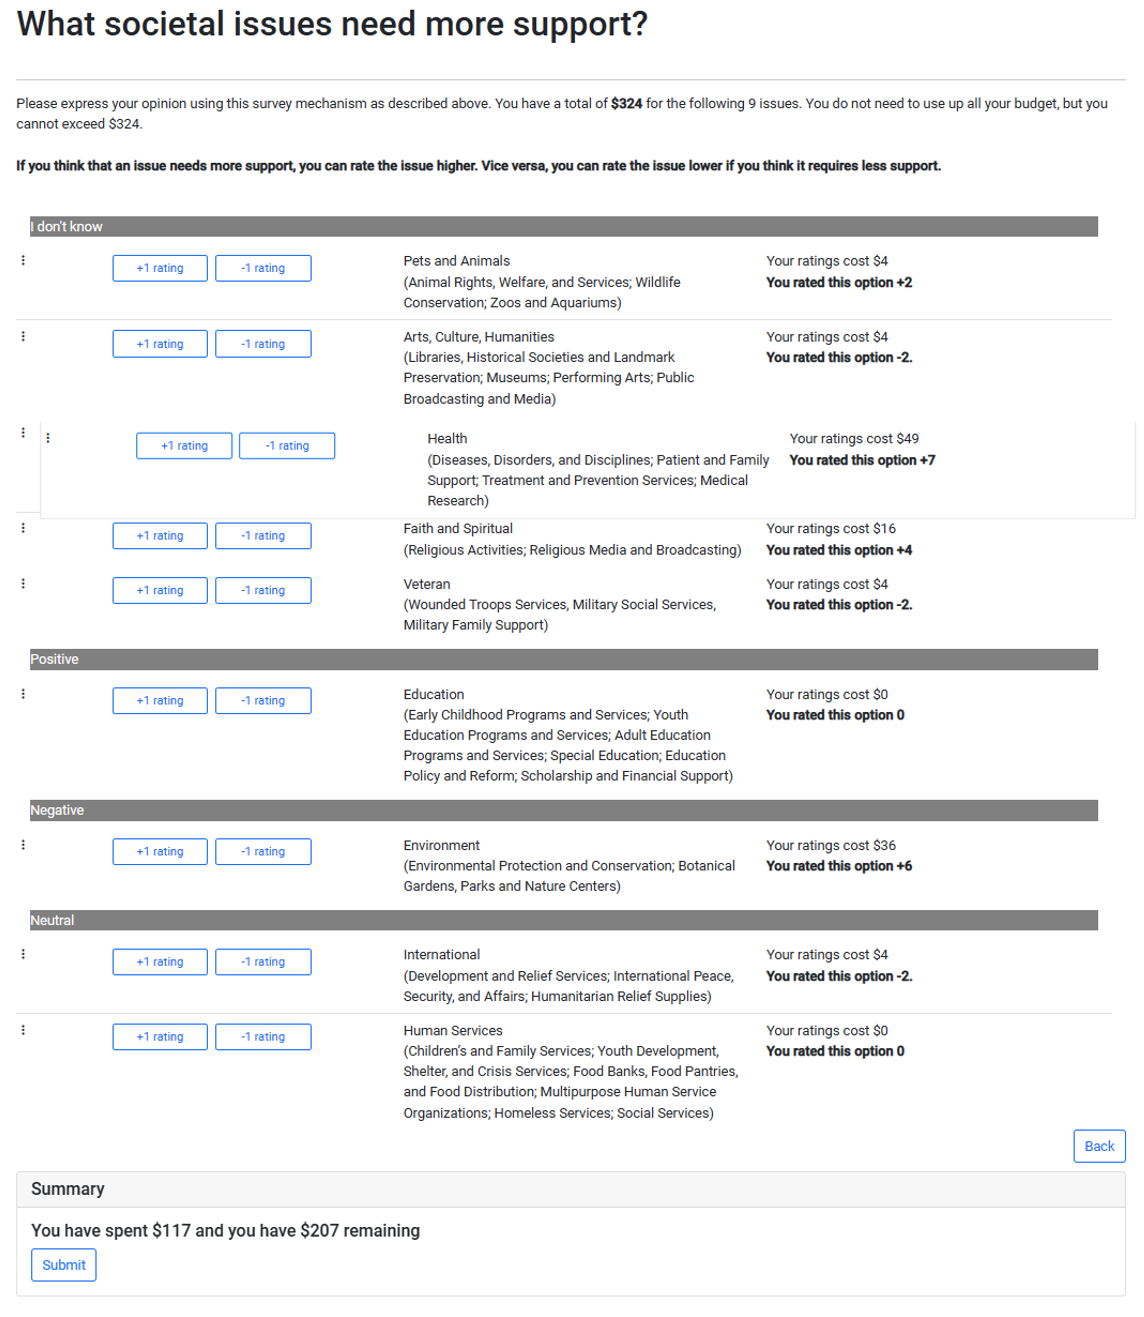
\includegraphics[width=\textwidth]{content/image/prototypes/4.2_grouping_vote.png}
        \caption{The Voting Interface: Voting controls appear on the left side of each option, showing the current votes and associated costs on the right. A budget summary is stuck at the bottom of the screen.}
        \label{fig:qv_org_p2}
    \end{subfigure}
    \caption{Organize-then-Vote Prototype: The goal of this prototype is to encourage participants at deriving finer grain categories among options before voting. Survey respondents first organize their thoughts into categories, then vote on the options.}
    \label{fig:qv_org}
\end{figure}

\subsubsection{Prototype 3: Organize-then-Vote}
Figure~\ref{fig:qv_org} shows the last prototype where we built on the previous takeaway by providing finer-grain groupings and creating a clear connection between option organization and voting position. Specifically, we provided three categories: Positive, Negative, and Neutral. Initially, respondents see all options under the section labeled 'I don't know,' which includes only the option descriptions. We ask respondents to move these options into the categories below. Voting controls and information appear on each option once respondents move to the subsequent page, forming a clear connection between option groups, positions, and voting controls.

Feedback indicated that survey respondents are comfortable with the two-phase organize-then-vote design, demonstrating it as a central strategy for our interface development. However, several areas for enhancement were identified: First, the dragging and dropping mechanism in the organization phase is cumbersome and may inadvertently suggest a ranking process, contrary to our intentions. Second, placing unorganized options at the top of the voting list is counterintuitive. Third, the voting controls are disconnected from the option summaries, dividing attention between the left and right sides of the screen. These insights guided refinements in the final two-phase interface, adhering to the two-phase organize-then-vote design framework.



\section{List of Options}
\label{sec:charityList}
We provide the full list of options presented on the survey.

\begin{itemize}
    \item \textbf{Animal Rights, Welfare, and Services:} Protect animals from cruelty, exploitation and other abuses, provide veterinary services and train guide dogs.
    \item \textbf{Wildlife Conservation:} Protect wildlife habitats, including fish, wildlife, and bird refuges and sanctuaries.
    \item \textbf{Zoos and Aquariums:} Support and invest in zoos, aquariums and zoological societies in communities throughout the country.
    \item \textbf{Libraries, Historical Societies and Landmark Preservation:} Support and invest public and specialized libraries, historical societies, historical preservation programs, and historical estates.
    \item \textbf{Museums:} Support and invest in maintaining collections and provide training to practitioners in traditional arts, science, technology, and natural history.
    \item \textbf{Performing Arts:} Support symphonies, orchestras, and other musical groups; ballets and operas; theater groups; arts festivals; and performance halls and cultural centers.
    \item \textbf{Public Broadcasting and Media:} Support public television and radio stations and networks, as well as providing other independent media and communications services to the public.
    \item \textbf{Community Foundations:} Promote giving by managing long-term donor-advised charitable funds for individual givers and distributing those funds to community-based charities over time.
    \item \textbf{Housing and Neighborhood Development:} Lead and finance development projects that invest in and improve communities by providing utility assistance, small business support programs, and other revitalization projects.
    \item \textbf{Jewish Federations:} Focus on a specific geographic region and primarily support Jewish-oriented programs, organizations and activities through grantmaking efforts
    \item \textbf{United Ways:} Identify and resolve community issues through partnerships with schools, government agencies, businesses, and others, with a focus on education, income and health.
    \item \textbf{Adult Education Programs and Services:} Provide opportunities for adults to expand their knowledge in a particular field or discipline, learn English as a second language, or complete their high school education.
    \item \textbf{Early Childhood Programs and Services:} Provide foundation-level learning and literacy for children prior to entering the formal school setting.
    \item \textbf{Education Policy and Reform:} Promote and provide research, policy, and reform of the management of educational institutions, educational systems, and education policy.
    \item \textbf{Scholarship and Financial Support:} Support and enable students to obtain the financial assistance they require to meet their educational and living expenses while in school.
    \item \textbf{Special Education:} Provide services, including placement, programming, instruction, and support for gifted children and youth or those with disabilities requiring modified curricula, teaching methods, or materials.
    \item \textbf{Youth Education Programs and Services:} Provide programming, classroom instruction, and support for school-aged students in various disciplines such as art education, STEM, outward bound learning experiences, and other programs that enhance formal education.
    \item \textbf{Botanical Gardens, Parks, and Nature Centers:} Promote preservation and appreciation of the environment, as well as leading anti-litter, tree planting and other environmental beautification campaigns.
    \item \textbf{Environmental Protection and Conservation:} Develop strategies to combat pollution, promote conservation and sustainable management of land, water, and energy resources, protect land, and improve the efficiency of energy and waste material usage.
    \item \textbf{Diseases, Disorders, and Disciplines:} Seek cures for diseases and disorders or promote specific medical disciplines by providing direct services, advocating for public support and understanding, and supporting targeted medical research.
    \item \textbf{Medical Research:} Devote and invest in efforts on researching causes and cures of disease and developing new treatments.
    \item \textbf{Patient and Family Support:} Support programs and services for family members and patients that are diagnosed with a serious illness, including wish granting programs, camping programs, housing or travel assistance.
    \item \textbf{Treatment and Prevention Services:} Provide direct medical services and educate the public on ways to prevent diseases and reduce health risks.
    \item \textbf{Advocacy and Education:} Support social justice through legal advocacy, social action, and supporting laws and measures that promote reform and protect civil rights, including election reform and tolerance among diverse groups.
    \item \textbf{Development and Relief Services:} Provide medical care and other human services as well as economic, educational, and agricultural development services to people around the world.
    \item \textbf{Humanitarian Relief Supplies:} Specialize in collecting donated medical, food, agriculture, and other supplies and distributing them overseas to those in need.
    \item \textbf{International Peace, Security, and Affairs:} Promote peace and security, cultural and student exchange programs, improve relations between particular countries, provide foreign policy research and advocacy, and United Nations-related organizations.
    \item \textbf{Religious Activities:} Support and promote various faiths.
    \item \textbf{Religious Media and Broadcasting:} Support organizations of all faiths that produce and distribute religious programming, literature, and other communications.
    \item \textbf{Non-Medical Science \& Technology Research:} Support research and services in a variety of scientific disciplines, advancing knowledge and understanding of areas such as energy efficiency, environmental and trade policies, and agricultural sustainability.
    \item \textbf{Social and Public Policy Research:} Support economic and social issues impacting our country today, educate the public, and influence policy regarding healthcare, employment rights, taxation, and other civic ventures.
\end{itemize}

\section{Cognitive Demand Tables}
Here we provide the full qualitative analysis table.

\subsection{Mental Demand Table}
\label{apdx:mental_table}
\begin{table}[h]
   \caption{This table lists all the causes participants mentioned as contributing to their Mental Demand. The shaded cells represent the percentage of participants citing each source of mental demand, allowing for comparison within columns. The abbreviations are: ST (Short Text Interface), SI (Short Two-phase Interface), LT (Long Text Interface), and LI (Long Two-phase Interface). Short and Long refer to the sum across both interfaces; Text and Inter refer to the sum across both survey lengths. We include Sparklines for comparisons across these experiment groups.}
    \label{tbl:mental}
    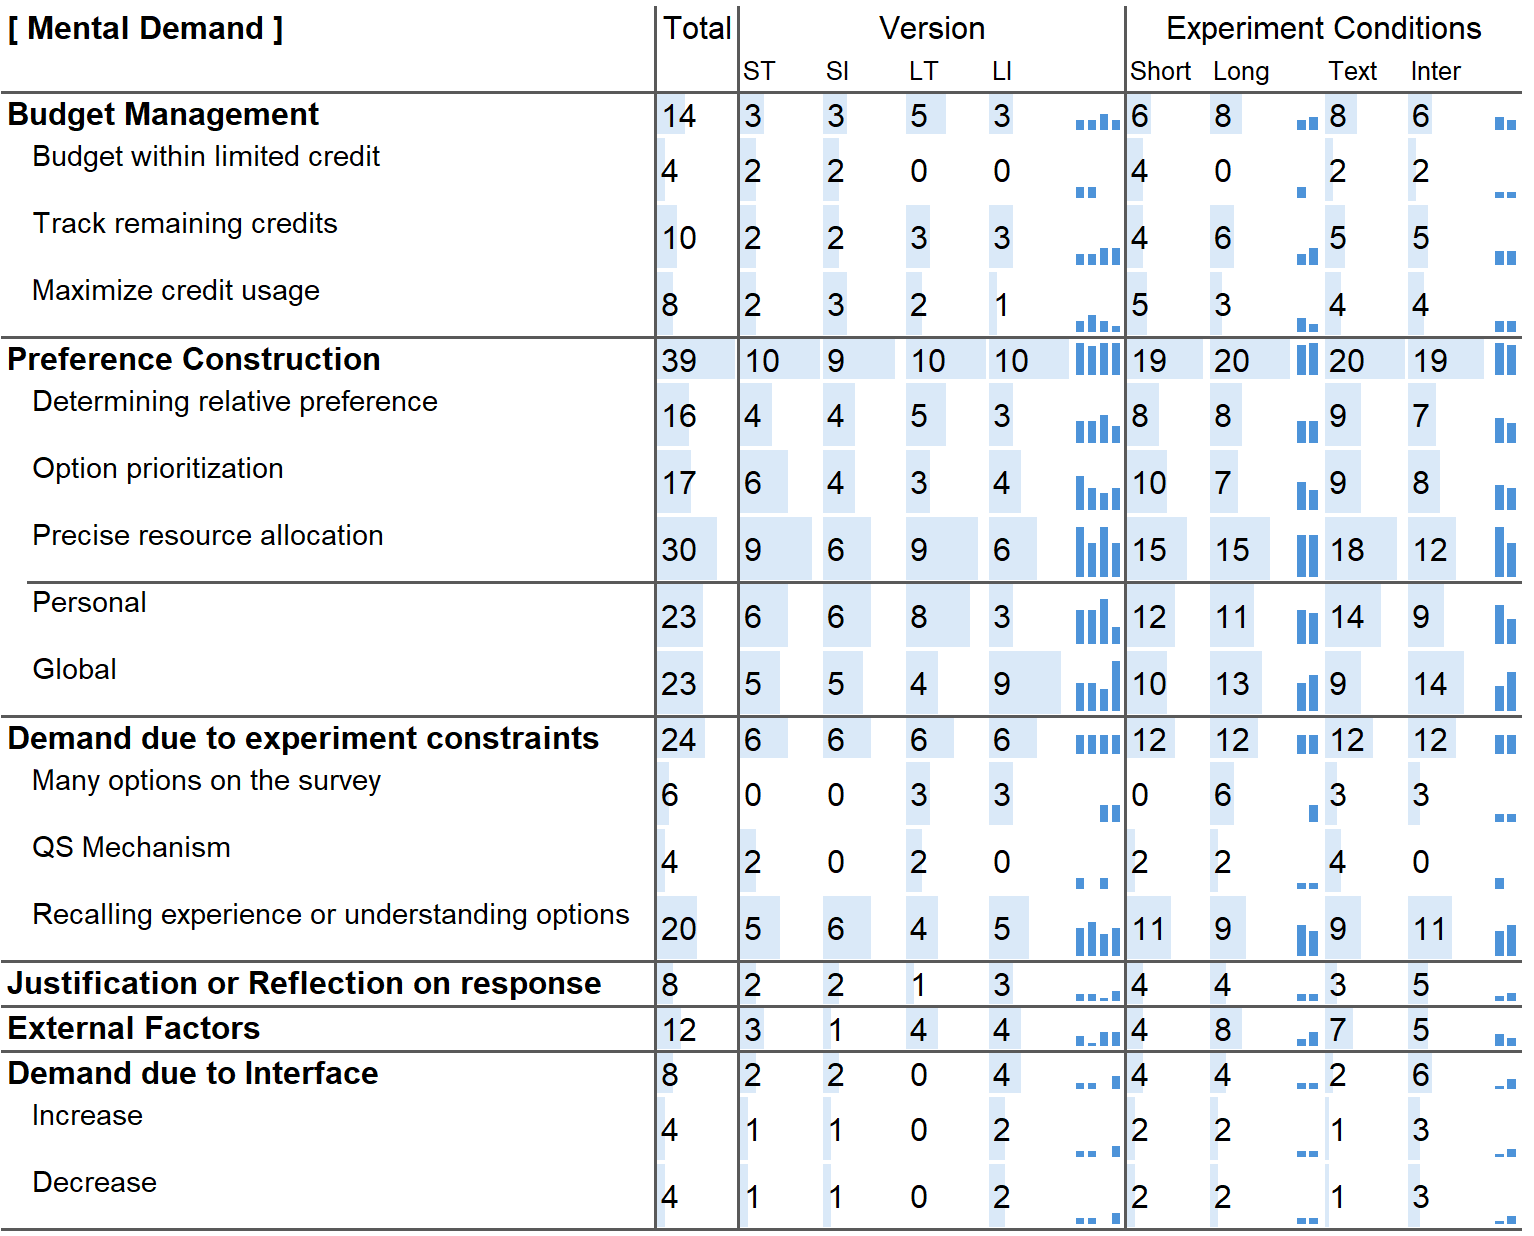
\includegraphics[width=\linewidth]{content/image/cog/mental_table.png}
\end{table}

\subsection{Physical Demand Table}
\label{apdx:physical_table}
\begin{table}[H]
    \caption{Physical Demand Causes: Most participants expressed little or no physical demand. Results reflected that participants in the long two-phase interface required more actions, hence the higher mention of mouse usage as a source.}
    \label{tbl:physical}
    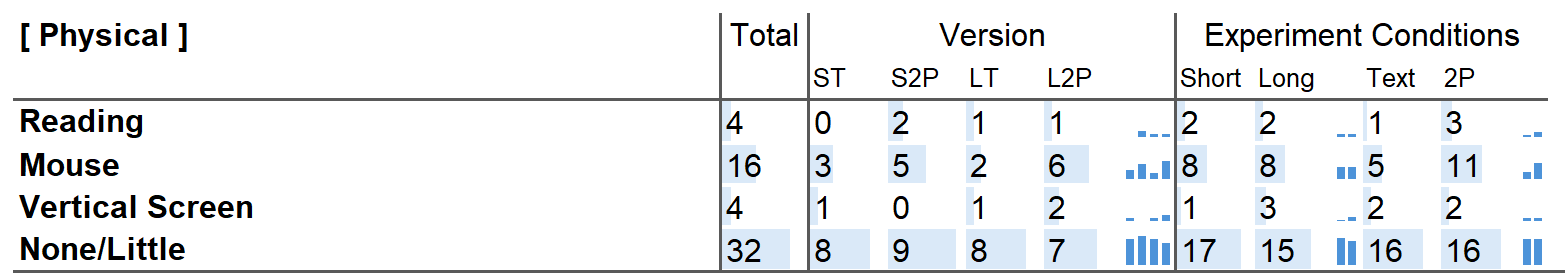
\includegraphics[width=\linewidth]{content/image/cog/physical_table.png}
\end{table}

\subsection{Performance Table}
\label{apdx:perf_table}
\begin{table}[H]
    \caption{Performance Causes: Most causes are shared across experiment conditions. We provided qualitative interpretations of their own perfornace assessments.}
    \label{tbl:physical}
    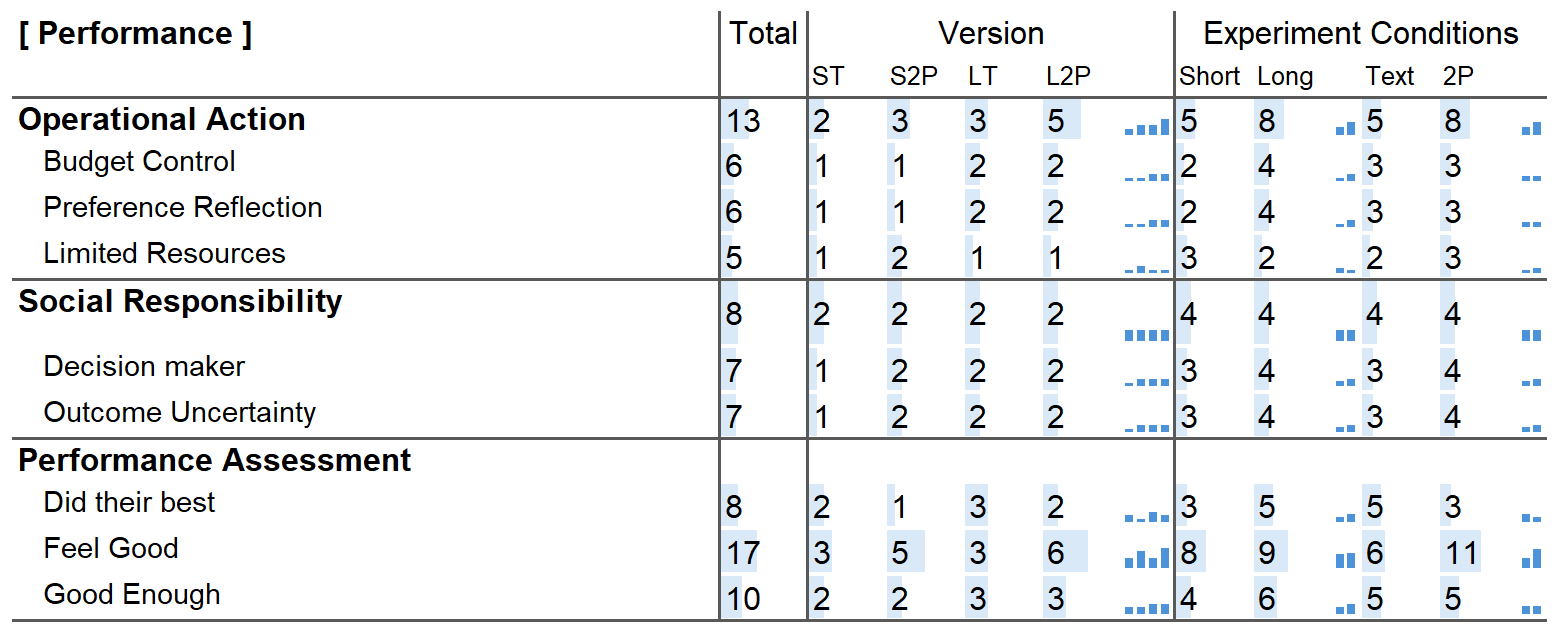
\includegraphics[width=\linewidth]{content/image/cog/perf_table.png}
\end{table}

\subsection{Temporal Demand Table}
\label{apdx:temporal_table}
\begin{table}[H]
    \caption{Temporal Demand Sources: Decision-making and Operational Tasks are the main causes. Participants framed their decision-making sources differently.}
    \label{tbl:temporal}
    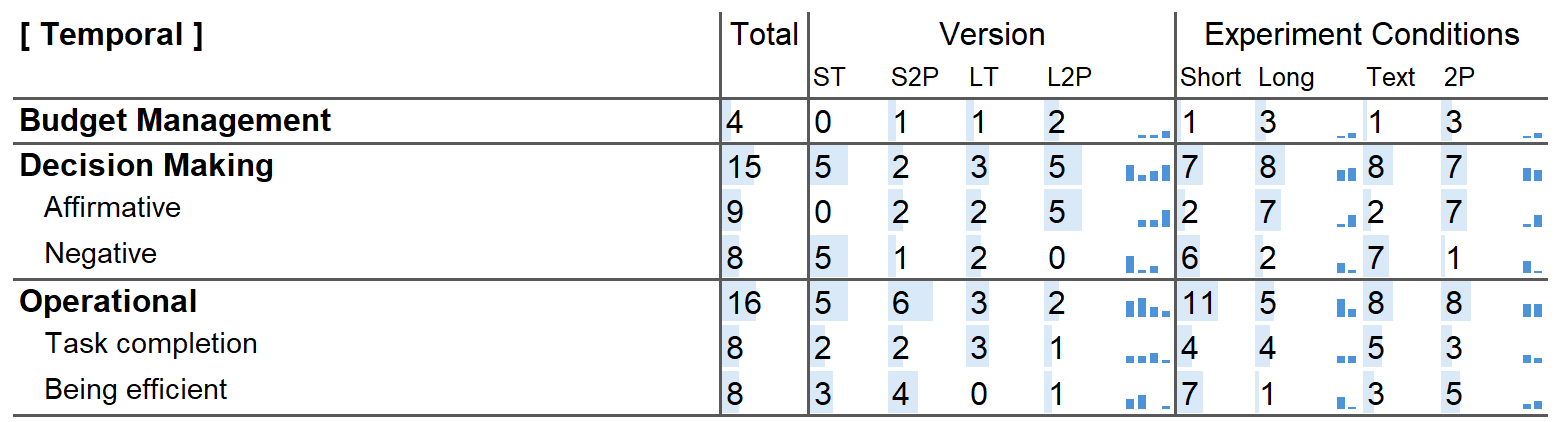
\includegraphics[width=\linewidth]{content/image/cog/temporal_table.png}
\end{table}

\subsection{Frustration Table}
\label{apdx:frus_table}
\begin{table}[H]
    \caption{Frustration Sources: needs to be updated with some new terms definitions for some of the columns.}
    \label{tbl:fustration}
    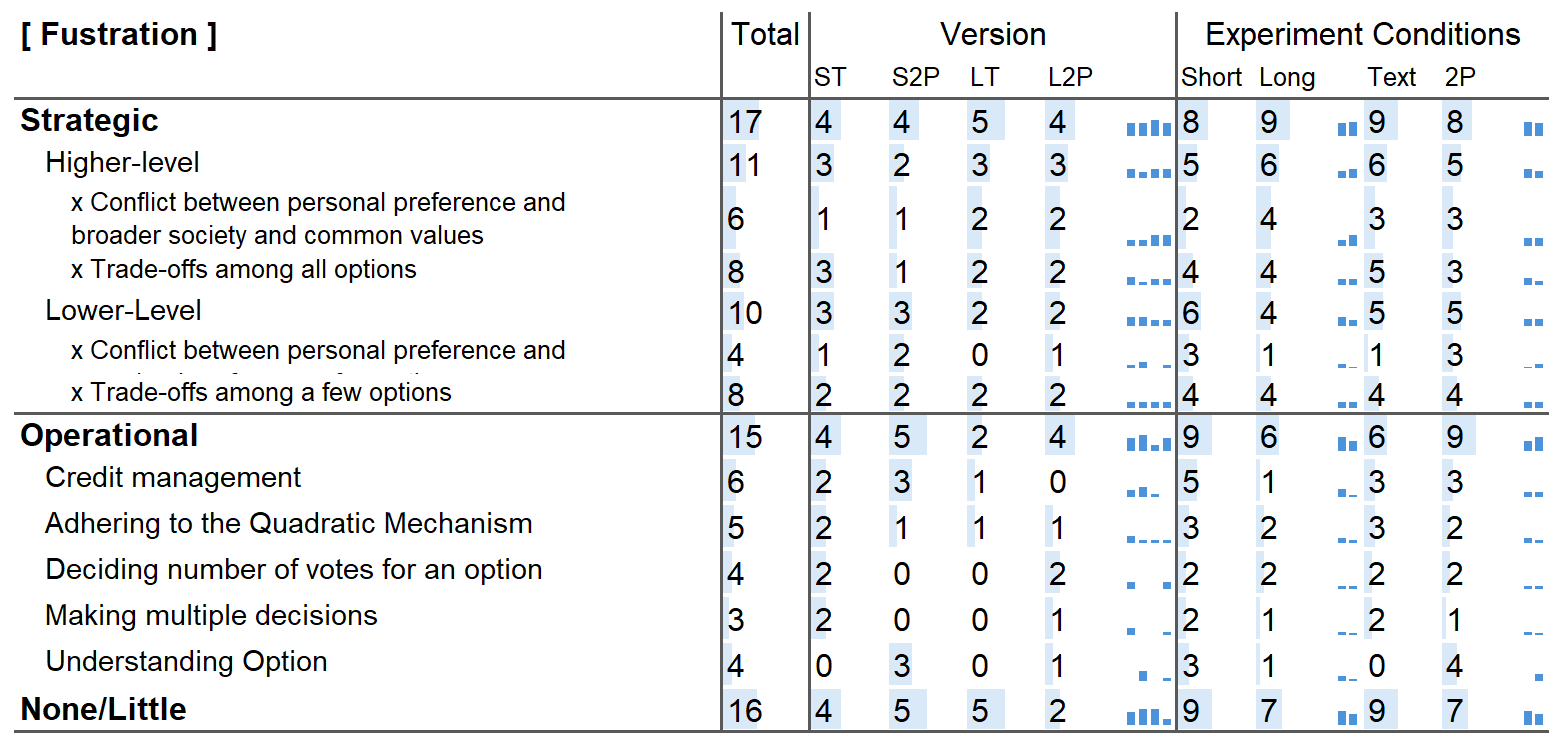
\includegraphics[width=\linewidth]{content/image/cog/fustration_table.png}
\end{table}

